\documentclass[slidestop,compress,mathserif,xcolor=svgnames,table]{beamer}

\usepackage[spanish]{babel}
\usepackage[utf8]{inputenc} % Ambos para solucin de asuntos de idioma.
\usepackage{amsmath, amsfonts, amssymb} % Matemticas varias.
\usepackage{longtable} % Tabla larga necesaria para el apndice de simbologa.
%\usepackage{multimedia}
\usepackage{movie15}
\usepackage{enumitem}

\setitemize{leftmargin=*}
\setitemize[1]{label=\tiny$\blacksquare$}
\setitemize[2]{label=\tiny$\bullet$}
\setitemize[3]{label=\tiny$\bullet$}
% \setbeamertemplate{sections in toc}[ball]

% --- Arreglos varios para la inclusion de imgenes
\usepackage{subfigure}
\DeclareGraphicsExtensions{.png,.jpg,.pdf,.mps,.gif,.bmp}

% ================= CONFIGURACIN DEL BEAMER ====================
% ===============================================================
\mode<presentation>{
% \usepackage{beamerthemeclassic}
% \setbeameroption{show notes}
% \setbeameroption{hide notes}
\setbeameroption{notes on second screen}
% \setbeamercovered{transparent}

% \usetheme{Warsaw}
% \usetheme{Frankfurt}
% \usetheme{Berlin}
% \usetheme{Madrid}
% \usetheme{Antibes}
% \usetheme{Darmstadt}
% \usetheme{Marburg}
% \usetheme{CambridgeUS}
% \usetheme{PaloAlto}
% \usetheme{AnnArbor}
\usetheme{Warsaw}
% \usecolortheme{rose}
% \usecolortheme{lily}
% \usecolortheme{seahorse}
% \usecolortheme{fly}
% \usecolortheme[RGB={70,110,45}]{structure}	% verde primaveral
% \usecolortheme[RGB={100,12,20}]{structure}	% rojo sangre
% \usecolortheme[RGB={30,40,30}]{structure}	    % Luto
% \usecolortheme[RGB={160,230,70}]{structure}	% verde manzana Grand-Smith

% \beamertemplateshadingbackground{green!30}{white}
 
% \usefonttheme[onlymath]{serif}
% \usefonttheme{professionalfonts}
\usefonttheme{structurebold}

% \setbeamerfont{frametitle}{family=\rmfamily,shape=\scshape,size=\normalsize}
% \setbeamertemplate{frametitle}[default][center]
% \setbeamerfont{section number projected}{family=\rmfamily,series=\bfseries,size=\tiny}
\setbeamercolor{section number projected}{bg=white,fg=black}


}
% Make a TOC appear before every section
%\AtBeginSection[]{
%\begin{frame}
%	\tableofcontents[currentsection]
%\end{frame}
%}

\AtBeginNote{Notas:\par}


% ========================= COMANDOS ============================
% ===============================================================
\newcommand{\ket}[1]{|#1\rangle}
\newcommand{\bcol}{\begin{columns}[T]}
\newcommand{\ecol}{\end{columns}}
\newcommand{\col}[1][0.5]{\column{#1\textwidth}}
\newenvironment{itemize*}%
  {\begin{itemize}%
    \setlength{\topsep}{10pt}%
    \setlength{\itemsep}{0pt}%
    \setlength{\parskip}{10pt}}%
  {\end{itemize}
}

% =================== DATOS DEL DOCUMENTO =======================
% ===============================================================
\author{Gonzalo Gutiérrez, Matas Tailanián}
\date{19 de Octubre de 2012}
\title{\textit{Seguimiento de Tempo}}
\subtitle{Procesamiento digital de senales de audio\\Curso 2012}



% ===============================================================
% ===============================================================
% ================ COMIENZO DEL DOCUMENTO =======================
% ===============================================================
% ===============================================================



\begin{document}

% ========================= FRAME ===============================
% ===============================================================
\begin{frame}
  \titlepage
\end{frame}


\section{Gral}
% ========================= FRAME ===============================
% ===============================================================
\begin{frame}
\frametitle{IBT: Real tempo and Beat-Tracking system}

\begin{columns}

\column{2in}
\vspace{15pt}
\begin{figure}[h!]
  \begin{center}
  \includegraphics[width=1\textwidth]{./pics/bloques.png}
  \end{center}
  \vspace{-10pt}
  \caption{Diagrama de bloques}
  \label{fig:bloques}
\end{figure}

\column{2in}
\vspace{20pt}
\begin{itemize}
	\item \textbf{Feature Selection}\pause
	\item \textbf{Pre Tracking}\\\pause
  	\begin{itemize*}
	  \item Período
	  \item Fase
	  \item Agente\pause
	\end{itemize*}
	\item \textbf{Beat tracking}
\end{itemize}

\end{columns}
\end{frame}

\section{Pre-Tracking}
% ========================= FRAME ===============================
% ===============================================================
\begin{frame}
\frametitle{Pre Tracking}

\begin{columns}
\column{2in}
\vspace*{15pt}
\begin{scriptsize}
	\begin{itemize} \item \textbf{Período} \end{itemize}
	\begin{equation*}
		A(\tau) = \sum\limits_{n=0}^{m}SF(n)SF(n+\tau)
		\label{ec:autocorrelacion}
	\end{equation*}
	$SF$ es el flujo espectral suavizado para el \emph{frame} $n$
	\begin{equation*}
		\begin{cases}
		P_i = \arg\max_i \left\{ A(\tau) \right\}, & i=1,\dots, N\\
		A(\tau)>\delta \frac{rms(A(\tau))}{M} & 
		\end{cases}
		\label{ec:period}
	\end{equation*}
$\delta$ es un umbral determinado empíricamente y $M$ es un rango de tiempos definido entre [50,250] BPM.
\end{scriptsize}
\pause

\column{2in}
\vspace*{15pt}
\begin{scriptsize}
\begin{itemize} \item \textbf{Fase} \end{itemize}
Para cada $P_i$ estimado se generan varias hipótesis para la fase: $\phi_i^j$. Se supone fase y períodos constantes en cada ventana de análisis.\\

Se utiliza un \emph{template} de tren de pulsos para ver cuál ajusta mejor.\\[.5cm]
\pause
\begin{itemize} \item \textbf{Agentes} \end{itemize}
Para cada pareja $(P_i,\phi_i)$ se computa la suma de errores entre el template de tren de pulsos y los máximos del flujo espectral

\end{scriptsize}
\end{columns}

\end{frame}



\section{Beat-Tracking}
% ========================= FRAME ===============================
% ===============================================================
\begin{frame}
\frametitle{Beat Tracking}
\begin{scriptsize}
\vspace*{-10pt}
\begin{block}{Idea}
Supervisar flujo de entrada y mantener balance entre inercia y rapidez de la respuesta
\end{block} \pause
\end{scriptsize}

\begin{columns}
\column{2in}
\vspace*{-10pt}
\begin{scriptsize}

Niveles de toleracia: $T_{in}\in[T_{in}^l,T_{in}^r]$ y $T_{out}\in[T_{out}^l,T_{in}^l] \bigcup [T_{in}^r,T_{out}^r]$

\begin{figure}[h!]
  \begin{center}
  \vspace*{-10pt}
  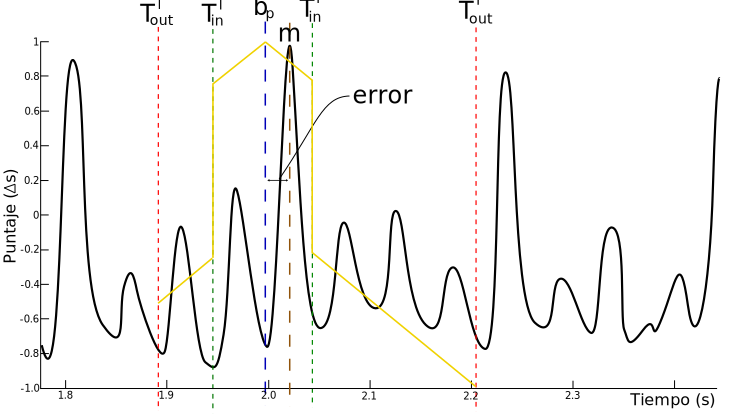
\includegraphics[width=.8\textwidth]{./pics/grafica.png}
  \end{center}
  \vspace{-10pt}
  \caption{Niveles de tolerancia}
  \label{fig:grafica}
\end{figure}
\pause
\end{scriptsize}
\column{2in}
\vspace*{-10pt}
\begin{scriptsize}

\begin{itemize} \item \textbf{$T_{in}\in[T_{in}^l,T_{in}^r]$} \end{itemize}
$$
\begin{cases}
P_i = P_i+0.25*error\\
\phi_i = \phi_i+0.25*error
\end{cases}
$$
\begin{itemize} \item \textbf{$T_{out}\in[T_{out}^l,T_{in}^l] \bigcup [T_{in}^r,T_{out}^r]$} \end{itemize}
El agente mantiene su período y fase y además crea 3 ``hijos'' variando dichos parámetros

\pause
\end{scriptsize}
\end{columns}
\vspace*{-10pt}
\begin{scriptsize}
\begin{block}{\emph{Agent Referee}}
Evalúa la distancia entre la predicción del \emph{beat} ($b_p$) y el máximo local ($m$) de $SF$. $P_m$ es el máximo período permitido
$$\begin{cases}
\Delta s = \left(1-\frac{|error|}{T^r_{out}} \right)\frac{P_i}{P_m}SF(m), & \exists m \in T_{in}\\
\Delta s = -\left(\frac{|error|}{T^r_{out}} \right)\frac{P_i}{P_m}SF(m), & \exists m \in T_{out}\\
\end{cases}$$
\end{block}
\end{scriptsize}

\end{frame}



\section{Plazos}
% ========================= FRAME ===============================
% ===============================================================
\begin{frame}
\frametitle{Tareas y plazos}
\begin{columns}
\column{2in}

\begin{scriptsize}

\begin{itemize}
	\item \textbf{Semana 12}
  	\begin{itemize*}
	  \item Profundización en la bibliografía seleccionada
	\end{itemize*}\pause
	\item \textbf{Semana 13}\\
	  	\begin{itemize*}
		  \item Determinar los programas e interfaces necesarias
		  \item Empezar a ``meter mano'' en el código
		\end{itemize*}\pause
	\item \textbf{Semana 14}\\
	  	\begin{itemize*}
		  \item Implementar las técnicas seleccionadas
		  \item Ajustar detalles
		\end{itemize*}\pause
\end{itemize}

\end{scriptsize}
\column{2in}
\begin{scriptsize}

\begin{itemize}
	\item \textbf{Semana 15}\\
	  	\begin{itemize*}
		  \item Ver la posibilidad y/o necesidad de implementar algún algoritmo para mejorar la performance (Filtro de Kalman)
		  \item Documentación y presentación
		\end{itemize*}
\end{itemize}

\end{scriptsize}
\end{columns}
\end{frame}






\section{Referencias}
% ===============================================================
% ========================= FRAME ===============================
% ===============================================================
\begin{frame}
\frametitle{Referencias:}
\begin{thebibliography}{99}
\begin{small}

\bibitem{bib:algo}Jo\~ao Lobato Oliveira, Fabien Gouyon, Luis Gustavo Martins, Luis Paulo Reis, IBT: A real time tempo and beat tracking system, In \emph{11th International Society for Music Information Retrieval Conference, ISMIR}, 2010.

\bibitem{bib:asdf}S. Dixon. Automatic extraction of tempo and beat from
expressive performances. In \emph{Journal of New Music Research, 30(1):39–58}, 2001.

\bibitem{bib:otra_cosa}S. Dixon. Onset detection revisited. In \emph{in Proceedings of the 9th International Conference on Digital Audio Effects}, pages 133–13, Montreal, Canada, 2006.

\bibitem{bib:y_asi}F. Gouyon, P. Herrera, and P. Cano. Pulse-dependent analyses of percussive music. In \emph{AES 22nd International Conference on Virtual}, Synthetic and Entertainment Audio, 2002.

\end{small}
\end{thebibliography}
\end{frame}

\end{document}





% ========================= FRAME ===============================
% ===============================================================
\begin{frame}
\frametitle{Title}
\begin{columns}
\column{2in}
\vspace*{-15pt}
\begin{scriptsize}


\begin{block}{title of the bloc}
bloc text
\end{block}
\begin{exampleblock}{title of the bloc}
bloc text
\end{exampleblock}
\begin{alertblock}{title of the bloc}
bloc text
\end{alertblock}


\end{scriptsize}
\column{2in}
\begin{scriptsize}

\begin{itemize}
	\item \textbf{Item 1}:\pause
  	\begin{itemize*}
	  \item subitem 1 \pause
	  \item subitem 2 \pause
	  \item subitem 3 \pause
	\end{itemize*}
	\item \textbf{Item 2}
\end{itemize}

\end{scriptsize}
\end{columns}
\end{frame}



% ================ FRAME TPICO CON FIGURA ======================
% ===============================================================

\begin{frame}
\frametitle{Qu es un Parcial?}

\begin{columns}

\column{2in}
\vspace{-25pt}
\begin{figure}[h!]
  \begin{center}
  \includegraphics[width=.85\textwidth]{./Pics/Espectrograma_ejemplo.jpg}
  \end{center}
  \vspace{-10pt}
  \caption{Espectrograma}
  \label{fig:espectrograma_ejemplo}
\end{figure}

\column{2in}
\begin{itemize}
	\item \textbf{Item 1}:\pause
  	\begin{itemize*}
	  \item subitem 1 \pause
	  \item subitem 2 \pause
	  \item subitem 3 \pause
	\end{itemize*}
	\item \textbf{Item 2}
\end{itemize}

\end{columns}
\end{frame}




% ======================== FIGURAS ==============================
% ===============================================================

\begin{figure}[h!]
	\centering
	\includegraphics[width=0.75\textwidth]{./Pics/		.eps}
	\caption{		}
	\label{fig:		}
\end{figure}

\begin{figure} [h!]
  \centering
  \subfloat[caption 1]{\label{fig:		}
  		\includegraphics[width=0.45\textwidth]
  			{./Pics/		.eps}}
  \subfloat[caption 2]{\label{fig:		} 
  		\includegraphics[width=0.45\textwidth]
  			{./Pics/ 		.eps}}
  \caption{Caption general}
  \label{fig:	label general	}
\end{figure}

\begin{wrapfigure}{l}{0.6\textwidth}
  \vspace{-20pt}
  \begin{center}
    \includegraphics[width=0.45\textwidth]
    	{./Pics/		.eps}
  \end{center}
  \vspace{-20pt}
  \caption{		}
  \label{ 		}
  \vspace{-10pt}
\end{wrapfigure}

\begin{figure} [h!]
  \begin{center}
    \begin{tabular}{cc}
      \resizebox{50mm}{!}
      	{\includegraphics{./Pics/ 	.eps}} &
      \resizebox{50mm}{!}
      	{\includegraphics{./Pics/	.eps}} \\
      \resizebox{50mm}{!}
      	{\includegraphics{./Pics/	.eps}} &
      \resizebox{50mm}{!}
      	{\includegraphics{./Pics/	.eps}} \\
    \end{tabular}
    \caption{ 		}
    \label{ 		}
  \end{center}
\end{figure}
